\chapter[Código]{Código}
\label{Chap5}

\section{Creación de Spiders}
Una vez instalado Scrapy, en nuestro directorio escogido escribimos el siguiente comando para generar un nuevo proyecto de Scrapy.

\begin{verbatim}
	scrapy startproject miproyecto
\end{verbatim}

Nos creara un nuevo directorio con el siguiente contenido.

\begin{figure} [h!]
	\centering
	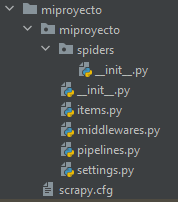
\includegraphics[width=0.3\textwidth]{fig/estructura_proyecto_scrapy.png}
	\caption[Estructura del proyecto recién creado]{Estructura del proyecto recién creado}
	\label{fig:ej11}
\end{figure}

Primero entraremos en el directorio recientemente creado y luego ejecuteremos el comando encargado de crear la Spider.

\begin{verbatim}
	cd miproyecto
	scrapy genspider mispider webausar.com
\end{verbatim}

En caso de no especificar el protocolo usado por la web Scrapy asumirá que usa HTTPS.
\newline
Tras ejecutar el comando la Spider habrá sido generada dentro de la carpeta spiders.

\begin{figure} [h!]
	\centering
	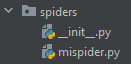
\includegraphics[width=0.3\textwidth]{fig/primera_spider.png}
	\caption[Directorio de almacenamiento de las Spider]{Directorio de almacenamiento de las Spider}
	\label{fig:ej12}
\end{figure}

Una vez abierto el archivo vemos que dispone del siguiente código.

\begin{lstlisting}[language=Python, caption={Spider recién generada}]
	import scrapy
	
	
	class MispiderSpider(scrapy.Spider):
		name = "mispider"
		allowed_domains = ["webausar.com"]
		start_urls = ["https://webausar.com"]
	
	def parse(self, response):
		pass
\end{lstlisting}

Como podemos ver Scrapy usa una programación orientada a objetos, siendo cada Spider una clase representada dentro del proyecto.\newline
Analizando las variables definidas vemos las siguientes, name, nombre por el que debemos referenciar la Spider a la hora de ejecutarla; allowed\_domains, indica que dominios podemos visitar, negando la entrada a cualquier dominio que no este definido en ella, es importante no especificar protocolo, de esta manera funcionara para cualquier web ya sea HTTP como HTTPS que pertenezca a ese dominio, de lo contrario se limitara al protocolo indicado; start\_urls, URL inicial sobre la que se hará la request de petición de datos.\newline
El método parse es aquel al que se envía la respuesta obtenida de la web, para realizar el filtrado de la información, quedándote unicamente con la deseada. Este método es invocado automáticamente por la Spider, sin necesidad real de hacerlo tu manualmente.

\subsection{Proceso de obtención de datos}
Para poder realizar es la extracción de los datos, primero debemos ir a la web deseada e inspeccionar su estructuración. Para ello como ejemplo vamos a usar la web de aemet.\newline

\begin{figure} [H]
	\centering
	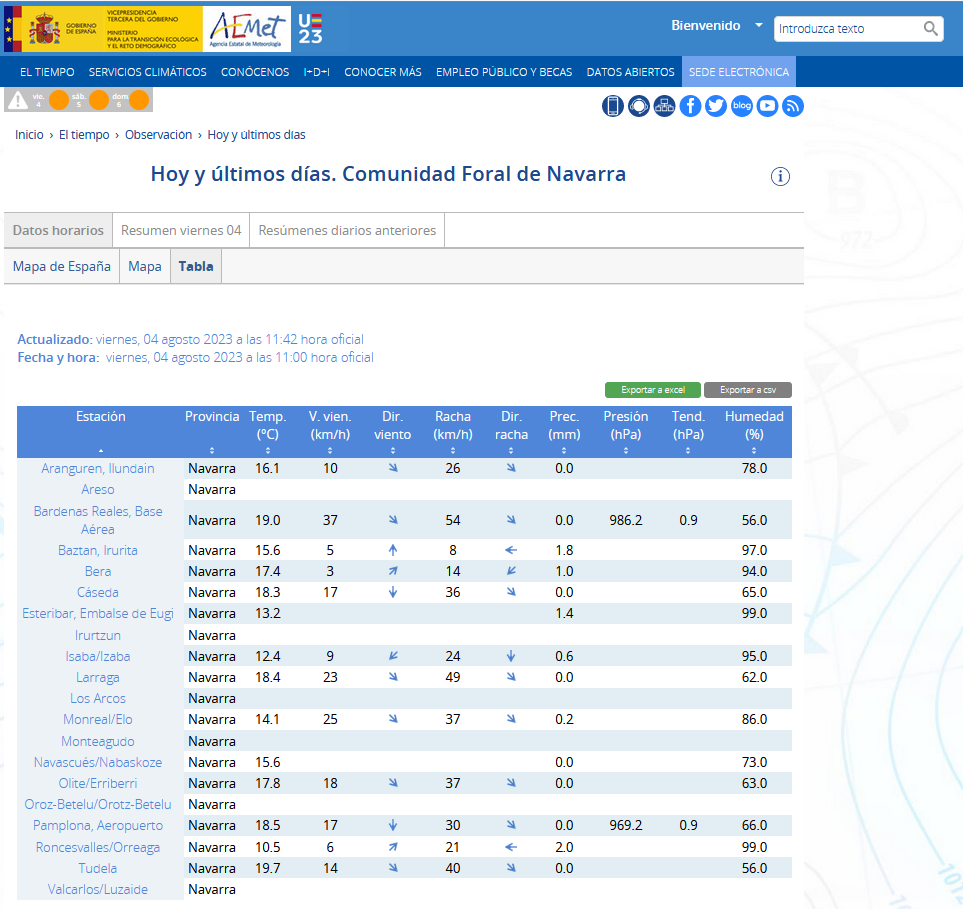
\includegraphics[width=0.8\textwidth]{fig/code_aemet.png}
	\caption[URL de inicio para obtener los códigos de las estaciones de Aemet]{Web de Aemet para obtención de datos}
	\label{fig:ej13}
\end{figure}

Una vez encontrada la web deseada, accediendo mediante el F12 a la herramienta de inspección, buscamos el elemento representativo del dato deseado. En nuestro caso queremos obtener tanto el nombre como el código de la estación. Ambos se encuentran en el mismo elemento que forma la primera columna de la tabla.\newline

\begin{figure} [H]
	\centering
	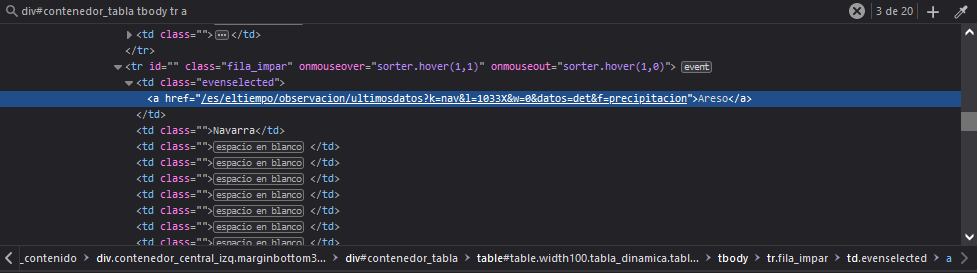
\includegraphics[width=0.9\textwidth]{fig/inspector.png}
	\caption[Inspector de webs de Chrome]{Inspector de webs}
	\label{fig:ej14}
\end{figure}

Como en este caso es posible filtrar fácilmente los datos, los obtendremos todos directamente, aunque lo más común sería obtener las filas primero para luego iterar por cada una de ellas. Para obtenerlos podemos hacerlo mediante el selector de XPath como con el de CSS.\newline

\begin{verbatim}
	rows = response.xpath('//div[@id="contenedor_tabla"]/table/tbody/tr/td/a')
	ó
	rows = response.css("div#contenedor_tabla tbody tr a")
\end{verbatim}

Esto nos devuelve una lista de objetos tipo Selector, cosa que nos permite conforme vamos iterando por cada elemento volver a usar un selector para filtrar unicamente los datos deseados. En nuestro caso.

\begin{verbatim}
	path = rows[i].xpath("@href").get()
	name = rows[i].xpath("./text()").get()
	ó
	path = rows[i].css("*::attr(href)").get()
	name = rows[i].css("*::text").get()
\end{verbatim}

De esta forma, mediante el uso de la función get(), pasamos de tener un objeto Selector a un String. El uso de get() sobre una lista devuelve el primer elemento, en caso de querer transformar toda la lista el método a usar es getall().\newline
\newline
Finalmente, como de la URL obtenida,
\begin{verbatim}
	'/es/eltiempo/observacion/ultimosdatos?k=nav&l=9263X&w=0&datos=det&f=precipitacion'
\end{verbatim}
solo nos interesa el código de la estación (parámetro l de la query), lo filtraremos.
\begin{verbatim}
	code = path.split('&')[1].split('=')[1]
\end{verbatim}

\subsection{Guardado de datos}
Scrapy almacena todos los datos en forma de múltiples diccionarios, tantos como webs usadas. Para acceder a esta información Scrapy nos proporciona dos alternativas, el uso de Items junto a ItemLoaders, siendo clases especificas de Scrapy o, mediante la palabra reservada yield de Python, siendo esta la opción elegida debido a su fácil implementación.
De esta forma escribiremos.
\begin{lstlisting}[language=Python, caption={Guardar datos}]
	yield {
		'estacion': name,
		'codigo': path.split('&')[1].split('=')[1],
	}
\end{lstlisting}
Actualmente si se ejecuta la Spider nos imprimiría los datos obtenidos por pantalla, aunque pueden ser almacenados en un fichero tanto CSV como JSON, a la hora de ejecutar la Spider añadiendo en el comando "-o nombre.csv ó -o nombre.json".\newline
Para un uso ligero de forma manual esa alternativa es más que suficiente, pero en nuestro caso, al querer ejecutarlas de forma automática mediante el uso de Runners, debemos implementar una variable llamada custom\_settings para cada una de las Spider. Esta permite, sin la necesidad de modificar el archivo settings.py, añadir configuraciones o dependencias independientes en las Spiders.

\begin{lstlisting}[language=Python, caption={Confugurar guardado en JSON}]
	custom_settings = {
		'FEEDS': {
			'JSONs/RawCode/codigos_aemet.json': {
				'format': 'json',
				'encoding': 'utf-8',
				'overwrite': True,
			}
		}
	}
\end{lstlisting}
Con esto indicamos que, en la ruta especificada, nos almacene un fichero JSON utf-8 y, que cada vez que se llame a esta Spider sobre-escriba el fichero anterior.

\subsection{Spider básica}
Una vez obtenemos los datos y los podemos almacenar, ya estaria nuestra Spider básica terminada.
\begin{lstlisting}[language=Python, caption={Spider de ejemplo}]
	import scrapy
	
	
	class AemetCodeSpider(scrapy.Spider):
		name = "aemet_code"
		allowed_domains = ["www.aemet.es"]
		start_urls = ["https://www.aemet.es/es/eltiempo/observacion/"
		"ultimosdatos?k=nav&w=0&datos=det&x=h24&f=precipitacion"]
		custom_settings = {
			'FEEDS': {
				'JSONs/RawCode/codigos_aemet.json': {
					'format': 'json',
					'encoding': 'utf-8',
					'overwrite': True,
				}
			}
		}
	
	def parse(self, response):
		rows = response.css("div#contenedor_tabla tbody tr a")
		
		for row in rows:
		path = row.xpath("@href").get()
		name = row.xpath("./text()").get()
		code = path.split('&')[1].split('=')[1]
		
		yield {
			'estacion': name,
			'codigo': code,
		}
\end{lstlisting}

\subsection{Método start\_requests()}
El método start\_requests() es llamado de forma automática al iniciar la Spider, siendo el encargado de hacer la llamada a la web indicada en start\_urls y, una vez obtenidos los datos llamar a la función parse, todo mediante un objeto Request de Scrapy, el cual devolverá un objeto tipo HTMLResponse. En caso de querer alterar el funcionamiento de la Spider este es el método a sobre-escribir.\newline
Como en nuestro caso queremos obtener los datos de todas las estaciones dentro de un mismo dominio, reescribiremos la función para que recorra el JSON con los códigos de estas y, hacer una llamada por estación con Request.
El código quedaría de la siguiente manera.

\begin{lstlisting}[language=Python, caption={Sobre-escritura de start\_request()}]
	def start_requests(self):
		with open("JSONs/RawCode/codigos_aemet.json", encoding="utf-8") as f:
			data = json.load(f)
		for estacion in data:
			url = f'https://www.aemet.es/es/eltiempo/observacion"
			"/ultimosdatos?k=nav&l={estacion["codigo"]}&w=0&"
			"datos=det&x=&f=temperatura'
			yield scrapy.Request(url, self.parse)
\end{lstlisting}

Al definir la función de esta manera no es necesario declarar la variable start\_urls, por lo que siempre que necesitemos sobre-escribir la función, no usaremos la variable.

\subsection{Eliminar Log}
Cuando se verifique el correcto funcionamiento de la Spider es recomendable quitar el maximo numero de Log por pantalla posible, es por eso que, en el fichero settings.py escribiremos las siguientes lineas.

\begin{lstlisting}[language=Python, caption={Configurar LOG}]
	LOG_LEVEL = 'WARNING'
	LOG_ENABLED = False
\end{lstlisting}

\section{Spiders usadas}
Como se ha dicho anteriormente, para este proyecto se han creado cuatro proyectos de Scrapy, uno por cada web.

\subsection{Aemet}

\begin{lstlisting}[language=Python, caption={Code Spider}]
	import scrapy
	
	
	class AemetCodeSpider(scrapy.Spider):
		name = "aemet_code_spider"
		allowed_domains = ["www.aemet.es"]
		start_urls = ["https://www.aemet.es/es/eltiempo/observacion/"
		"ultimosdatos?k=nav&w=0&datos=det&x=h24&f=temperatura"]
		custom_settings = {
			'FEEDS': {
				'JSONs/RawCode/codigos_aemet.json': {
					'format': 'json',
					'encoding': 'utf-8',
					'overwrite': True,
				}
			}
		}
	
	def parse(self, response):
		rows = response.css("div#contenedor_tabla tbody tr a")
		
		for row in rows:
			path = row.xpath("@href").get()
			name = row.xpath("./text()").get()
			yield {
				'estacion': name,
				'codigo': path.split('&')[1].split('=')[1],
			}
\end{lstlisting}

Siendo esta la Spider usada como ejemplo no hay mucho más que comentar al respecto, se dedica a obtener los nombres y códigos de cada estación.

\begin{lstlisting}[language=Python, caption={Data Spider}]
	import json
	
	import scrapy
	
	
	class AemetDataSpider(scrapy.Spider):
		name = "aemet_data_spider"
		allowed_domains = ["www.aemet.es"]
		custom_settings = {
			'FEEDS': {
				'JSONs/RawData/datos_aemet.json': {
					'format': 'json',
					'encoding': 'utf-8',
					'overwrite': True,
				}
			}
		}
	
	def start_requests(self):
		with open("JSONs/RawCode/codigos_aemet.json", encoding="utf-8") as f:
			data = json.load(f)
		for estacion in data:
			url = f'https://www.aemet.es/es/eltiempo/observacion/"
			"ultimosdatos?k=nav&l={estacion["codigo"]}&w=0&"
			"datos=det&x=&f=temperatura'
			yield scrapy.Request(url, self.parse)
	
	def parse(self, response):
		latitud = response.css('abbr.latitude::text').get()
		longitud = response.css('abbr.longitude::text').get()
		estacion = response.css("a.separador_pestanhas").get()
		rows = response.css('tbody tr')
		
		datos = []
		for row in rows:
			dato = {
				'fecha y hora': row.xpath('./td[1]/text()').get() + ':00',
				'temperatura (C)': row.xpath('./td[2]/text()').get(),
				'humedad (%)': row.xpath('./td[10]/text()').get(),
				'precipitacion (mm)': row.xpath('./td[7]/text()').get(),
			}
			
			if dato['precipitacion (mm)'] != " ":
				datos.append(dato)
		
		yield {
			'coordenadas': latitud + ' | ' + longitud,
			'estacion': estacion.split('=')[3].split('&')[0],
			'datos': datos,
		}
\end{lstlisting}

Como vemos, la Spider de obtención de datos ya es un poco más compleja, necesitando sobre-escribir la función de start\_request(). También se puede observar como inicialmente todos los datos son almacenados en una lista antes de ser guardados, el motivo de esto es muy simple y, es que de no hacerlo solo recibiría el primer dato de entre todos los recogidos.\newline
A su vez dentro del bucle for se ha añadido un if para asegurarse de no guardar datos vacíos, pues puede darse el caso en el que la web aun no tenga el dato de precipitación a cierta hora pero si muestre esta franja horaria pues dispone de otros datos como pueden ser aquellos relacionados con el viento.\newline
Por otro lado, como las coordenadas son mostradas en la misma página que los datos, en vez de crear otra Spider específicamente para obtenerlos, se hace uso de esta con el fin de minimizar código y tiempo de ejecución.

\subsection{Chcantabrico}

\begin{lstlisting}[language=Python, caption={Code Spider}]
	import scrapy
	
	
	class ChcantabricoCodeSpider(scrapy.Spider):
		name = "chcantabrico_code_spider"
		allowed_domains = ["www.chcantabrico.es"]
		start_urls = ["https://www.chcantabrico.es/nivel-de-los-rios"]
		custom_settings = {
			'FEEDS': {
				'JSONs/RawCode/codigos_chcantabrico.json': {
					'format': 'json',
					'encoding': 'utf-8',
					'overwrite': True,
				}
			}
		}
	
	def parse(self, response):
		rows = response.xpath('//table[@class="tablefixedheader niveles"]/tbody/tr')
		
		for row in rows:
			codigoBusqueda = row.css('td.codigo::text').get()
			limites = row.css('table.umbrales_gr td.datos::text').getall()
			paths = row.xpath('./td/a/@href').getall()
			estaciones = row.xpath('./td/a/text()').getall()
		
			for i in range(len(limites)):
				if limites[i] == 'No definido':
					limites[i] = None
			
			yield {
				'estacion': estaciones[-3],
				'codigo': paths[-1].split("=")[-1],
				'codigoSecundario': codigoBusqueda,
				'seguimiento': limites[0],
				'prealerta': limites[1],
				'alerta': limites[2],
			}
\end{lstlisting}

Esta puede ser la Spider de obtención de códigos más compleja. esto se debe en parte por la estructuración de la web, mostrando una tabla con otra tabla integrada por cada una de las filas, como por la cantidad de información que dispone.\newline
El primer problema fue como obtener las filas de la tabla principal, pues en muchos de los intentos realizados no solo tomaba estas filas, si no que tomaba aquellas que formaban parte de las tablas incluidas es ellas también. Finalmente, aunque con el Selector CSS no lo logré, mediante Xpath fue posible filtrarlas.\newline
Otra cosa a mencionar es que Chcantabrico proporciona dos códigos por estación, uno referenciando a la estación en si, siendo el usado para posteriormente obtener las coordenadas, aquel que llamo codigoSecundario o codigoBusqueda mientras que, el segundo hace referencia a los datos como tal. Puesto que no todas las filas disponen de la misma cantidad de enlaces, se obtienen todos sabiendo que siempre el ultimo de ellos dispone del código deseado.\newline
Finalmente, dentro de la tabla secundaria, esta es la única web que llega a proporcionar los valores de seguimiento, pre-alerta y alerta del río, siendo estos una buena base para empezar con las predicciones de inundación. En caso de no estar definido el valor simplemente se indicará como None.

\begin{lstlisting}[language=Python, caption={Nivel Spider}]
	import io
	import json
	
	import pandas as pd
	import scrapy
	
	
	class ChcantabricoNivelSpider(scrapy.Spider):
		name = "chcantabrico_nivel_spider"
		allowed_domains = ["www.chcantabrico.es"]
		custom_settings = {
			'FEEDS': {
				'JSONs/RawData/datos_nivel_chcantabrico.json': {
					'format': 'json',
					'encoding': 'utf-8',
					'overwrite': True,
				}
			}
		}
	
	def start_requests(self):
		with open("JSONs/RawCode/codigos_chcantabrico.json", encoding="utf-8") as f:
			data = json.load(f)
		for estacion in data:
			params_nivel = {
				'p_p_id': 'GraficaEstacion_INSTANCE_wH0LL6jTUysu',
				'p_p_lifecycle': '2',
				'p_p_state': 'normal',
				'p_p_mode': 'view',
				'p_p_resource_id': 'downloadCsv',
				'p_p_cacheability': 'cacheLevelPage',
				'_GraficaEstacion_INSTANCE_wH0LL6jTUysu_cod_estacion': f'{estacion["codigo"]}',
				'_GraficaEstacion_INSTANCE_wH0LL6jTUysu_tipodato': 'nivel',
			}
			url = 'https://www.chcantabrico.es/evolucion-de-niveles'
			yield scrapy.FormRequest(url=url,
			method='GET',
			formdata=params_nivel,
			callback=self.parse,
			cb_kwargs={'estacion': estacion['codigo']}
			)
	
	def parse(self, response, estacion):
		if not response.text.startswith('-'):
			urlData = response.text
			rawData = pd.read_csv(io.StringIO(urlData), delimiter=';', encoding='utf-8', header=1)
			rawData.columns = ['fecha y hora', 'nivel (m)']
			parsedData = rawData.to_json(orient="records")
			
			yield {
				'estacion': estacion,
				'datos': json.loads(parsedData)
			}
\end{lstlisting}

\begin{lstlisting}[language=Python, caption={Pluviometric Spider}]
	import io
	import json
	
	import pandas as pd
	import scrapy
	
	
	class ChcantabricoPluvioSpider(scrapy.Spider):
		name = "chcantabrico_pluvio_spider"
		allowed_domains = ["www.chcantabrico.es"]
		custom_settings = {
			'FEEDS': {
				'JSONs/RawData/datos_pluvio_chcantabrico.json': {
					'format': 'json',
					'encoding': 'utf-8',
					'overwrite': True,
				}
			}
		}
	
	def start_requests(self):
		with open("JSONs/RawCode/codigos_chcantabrico.json", encoding="utf-8") as f:
			data = json.load(f)
		for estacion in data:
			params_pluvio = {
				'p_p_id': 'GraficaEstacion_INSTANCE_ND81Xo17PIZ7',
				'p_p_lifecycle': '2',
				'p_p_state': 'normal',
				'p_p_mode': 'view',
				'p_p_resource_id': 'downloadCsvPluvio',
				'p_p_cacheability': 'cacheLevelPage',
				'_GraficaEstacion_INSTANCE_ND81Xo17PIZ7_cod_estacion': f'{estacion["codigo"]}',
				'_GraficaEstacion_INSTANCE_ND81Xo17PIZ7_tipodato': 'pluvio',
			}
			url = 'https://www.chcantabrico.es/precipitacion-acumulada'
			yield scrapy.FormRequest(url=url,
			method='GET',
			formdata=params_pluvio,
			callback=self.parse,
			cb_kwargs={'estacion': estacion['codigo']}
			)
	
	def parse(self, response, estacion):
		if not response.text.startswith('-'):
			urlData = response.text
			rawData = pd.read_csv(io.StringIO(urlData), delimiter=';', encoding='utf-8', header=1)
			rawData.columns = ['fecha y hora', 'nivel (m)']
			parsedData = rawData.to_json(orient="records")
			
			yield {
				'estacion': estacion,
				'datos': json.loads(parsedData)
			}
\end{lstlisting}

Chacantabrico muestra datos tanto del nivel del río como de la precipitación, aunque lo hace en dos direcciones distintas, haciendo necesario el uso de dos Spiders.\newline
A su vez, como Chcantabrico no muestra los datos por pantalla, incluyendo un botón sobre el que pulsar para obtenerlos descargando un fichero CSV, en vez de hacer una request básica mediante la clase Request, vamos ha hacer uso de FormRequest para hacer una llamada GET, pudiendo simular la llamada a un formulario y obtener los datos que este devuelve. De esta forma, pasandole los parámetros necesarios en el argumento formdata a la URL indicada, podemos obtener los datos sin la necesidad de ningún CSV, simulando en cierto modo una llamada mediante cURL. Cabe mencionar que, Request devuelve un HTMLResponse y que, la respuesta que obtenemos de estas llamadas no es codigo HTML, por lo que, aun en caso de que llegue a ser posible usar Request, es más correcto el uso de FormRequest devolviendo un FormResponse para este tipo de casos.\newline
El uso del argumento cb\_kwargs sirve para enviar un mayor numero de argumentos a la función parse() de los que normalmente recibe, es por ello que la función parse() recibe un tercer argumento que hemos decidido llamar estación. En este caso para poder enviar a cada conjunto de datos recibidos el código de la estación a la que pertenecen, pues dentro de la respuesta obtenida solo se proporciona el nombre de esta.\newline
Dentro de la función parse() lo primero que se hace es comprobar que realmente se ha recibido una respuesta correcta, pues, aunque todas la estaciones disponen de datos del nivel del río, no todas disponen los de precipitación, el problema viene cuando a estas estaciones se les piden los datos, ya que en vez de enviar un error 404 como seria esperado, te devuelven una respuesta vacía iniciada por '-'. Una alternativa para deshacerse de esta comprobación sería eliminando aquellas estaciones que no proporcionen datos o filtrandolas para no hacer la llamada directamente, aunque esto no solo nos resultaría más complejo, si no que nos crearía el problema de que cada cierto tiempo habría que comprobar si alguna estación ha empezado a proporcionar datos para incluirla nuevamente en la lista de estaciones a las cuales hacer llamada.
